
    \documentclass{article}

    %  Русский язык

    \usepackage[T2A]{fontenc}			% кодировка
    \usepackage[utf8]{inputenc}			% кодировка исходного текста
    \usepackage[english,russian]{babel}	% локализация и переносы
    \usepackage{unicode-math}

    % Рисунки
    \usepackage{graphicx, float}
    \usepackage{wrapfig}


    \title{Wild wild west derivative counter}
    \author{Dodo}
    \date{November 2022}


    \begin{document}
    \maketitle
    
        Welcome to derivative calculator fella, let's have a look at ya. God, what da hell is dis shit, fella?
        Ok, ok, let's calculate this bullshit.

        \begin{center}
        $\clubsuit$~$\clubsuit$~$\clubsuit$
        \end{center}
    \begin{figure}[H] 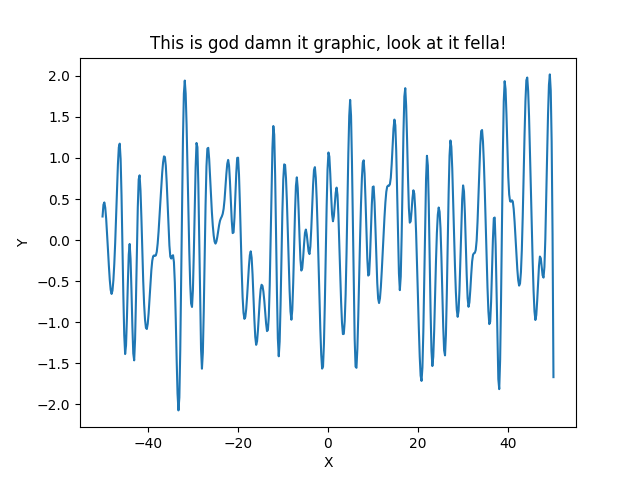
\includegraphics[scale=0.6]{function_graph.png} \end{figure}Alright fella, let's look wat we got:

\begin{equation}
{({cos({X})})\cdot({1})}
\end{equation}
\begin{center} $\clubsuit$~$\clubsuit$~$\clubsuit$ \end{center}